\tikzsetnextfilename{t_two_spines}
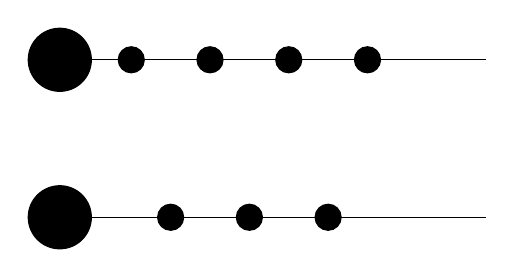
\begin{tikzpicture}

\draw (0, 0) node[left] {$S_2$} -- (5, 0);
\draw (0, 2) node[left] {$S_1$} -- (5, 2);

\tikzstyle{every node}+=[circle,draw,fill]

\node[circle,draw] (o1) at (1, 0) {};
\node[right of=o1] (o2) {};
\node[right of=o2] (o3) {};

\node (u1) at (0.5, 2) {};
\node[right of=u1] (u2) {};
\node[right of=u2] (u3) {};
\node[right of=u3] (u4) {};

\drawedges[bend right]{o1/o2,o1/o3,o2/o3}
\drawedges{o1/u1,o1/u2,o2/u2,o2/u3,o2/u4}
\drawedges[bend left]{u1/u4,u2/u3}

\end{tikzpicture}